\documentclass[t,aspectratio=169]{beamer}
\usepackage[utf8]{inputenc}
\usepackage[T1]{fontenc}
\usepackage{xcolor}
\usepackage{hyperref}
\usepackage{tikz}
\usepackage{tikz-cd}
\usepackage{pgfplots}
\pgfplotsset{compat=1.8}
\usepackage{adjustbox}
\usepackage{tabularx}
\usepackage{array}
\usepackage{fontspec}
\usefonttheme{serif} % default family is serif
\usepackage{hyperref}

\title{Multimodal MCMC with Replica Exchange and TensorFlow Probability}
\date{Bayesian Mixer London, Nov 30, 2020}
\author{Simeon Carstens, Tweag I/O}
\newcommand{\todo}{\textcolor{red}{\textbf{TODO}}}
\renewcommand{\d}{\mathrm{d}}
\newcommand{\btVFill}{\vskip0pt plus 1filll}
\setmainfont{Roboto}
\usetheme{tweag}

\begin{document}

\begin{frame}
  \titlepage
\end{frame}


\begin{frame}
  \frametitle{Your hosts}
  \begin{tcolorbox}[title=Simeon (presentation)]
    \begin{minipage}{0.3\textwidth}{
        \includegraphics[width=0.15\paperwidth]{images/simeon}}
    \end{minipage}
    \begin{minipage}{0.6\textwidth}
    \begin{itemize}
    \item background in computational biology
    \item Data Scientist at Tweag since 2019
    \item lives in Paris
    \end{itemize}
    \end{minipage}
  \end{tcolorbox}
\end{frame}


\begin{frame}
  \frametitle{Tweag I/O}
  Software innovation lab and consultancy based in Paris with employees all around the world and a strong focus on open-source software.\\
  \bigskip
  We specialize in
  \begin{itemize}
  \item software engineering, with a focus on functional programming
  \item DevOps, with a focus on reproducible software systems and builds
  \item data science
  \end{itemize}
  Key industries: finance, biotech, automotive\\
  \bigskip
  Need help with your project? Want to work with us?\\
  \bigskip
  \centering
  www.tweag.io\\
  \bigskip
  hello@tweag.io
\end{frame}


\begin{frame}
  \frametitle{What you're in for}
\end{frame}

\begin{frame}
  \frametitle{Multimodality}
  \begin{columns}
    \begin{column}{0.48\textwidth}
      Unimodal distribution:
      \includegraphics[width=0.8\textwidth]{images/unimodal}
    \end{column}
    \begin{column}{0.48\textwidth}
      Bimodal distribution:
      \includegraphics[width=0.8\textwidth]{images/bimodal}
    \end{column}
  \end{columns}
\end{frame}

\begin{frame}
  \frametitle{Multimodality: common occurences}
  \begin{description}
  \item[mixture models] \hfill \\
    For GMM parameterized by mixture weight $\theta$ and $\mu_1, \mu_2, \sigma$:
    \begin{equation*}
      p(\theta, \mu_1, \mu_2, \sigma|y) = p(1-\theta, \mu_2, \mu_1, \sigma|y)
    \end{equation*}
  \item[models invariant under reflections] \hfill \\
    e.g., biomolecular structure determination:
    \begin{equation*}
     L(\mathbf x_1, \ldots \mathbf x_N) = p(D|\mathbf x_1, \ldots \mathbf x_N) = L(\ldots, |\mathbf x_i - \mathbf x_j| \ldots)
    \end{equation*}
  \item[latent variable models] \hfill \\
    e.g., probabilistic PCA: symmetry w.r.t. rotation of latent variable coordinates
  % \item[overparameterized models]
  \end{description}
\end{frame}

\begin{frame}
  \frametitle{Refresher: Metropolis-Hastings}
  \begin{columns}
  \begin{column}{0.48\textwidth}
  \begin{tcolorbox}[fontupper=\small, title=Markov chain]
    Random process with
    \begin{equation*}
      p(x_{i+1}|x_i, x_{i-1}, \ldots, x_1) = p(x_{i+1}|x_i)
    \end{equation*}
    $\rightarrow$ a Markov chain has no ``memory''\\
    
    In some conditions: converges to a unique invariant distribution $\pi(x)$
  \end{tcolorbox}  
\end{column}
\begin{column}{0.48\textwidth}  
  \begin{tcolorbox}[fontupper=\small, title=Metropolis-Hastings algorithm]
    %\tcblower
    Construct Markov chain with invariant distribution $\pi(x)=p(x)$:
    \begin{enumerate}
    \item starting at state, $x_i$, propose a new state $x_{i+1}^*$ from $q(x_{i+1}^*|x_i)$
    \item calculate acceptance probability $p_{\mathrm{acc}}$
    \item draw $u \sim \mathcal U(0,1)$
    \item if $u < p_{\mathrm{acc}}$: $x_{i+1} = x_{i+1}^*$, else $x_{i+1} = x_i$
    \end{enumerate}
  \end{tcolorbox}
\end{column}
\end{columns}
\end{frame}

\begin{frame}{Metropolis (-Hastings)}
  Initialize with any state $x_0$\\
  \adjustbox{valign=t}{
  \begin{minipage}{0.45\linewidth}
    \par
    \noindent\phantom{\parbox{\linewidth}{%
    \begin{enumerate}
    \item calculate a proposal state $x_1^*$ by randomly perturbing $x_0$
    \item calculate acceptance probability
      \[p_\mathrm{acc}=\min\left(\frac{p(x_1^*)}{p(x_0)}, 1\right)\]
    \item with probability $p_\mathrm{acc}$, accept proposal state $x_1^*$ as the next state $x_1$, else copy $x_0$
    \end{enumerate}
    }}\par
    \vfill
    Sequence of states:\\
    $(x_0)$
  \end{minipage}}
  \hfill
  \adjustbox{valign=t}{
  \begin{minipage}{0.45\linewidth}
    \includegraphics[width=1.0\linewidth]{images/rwmc/03}
  \end{minipage}}
  \btVFill  
  \hfill \scriptsize Metropolis et al., J. Chem. Phys (1953); Hastings, Biometrika (1970)\smallskip
\end{frame}


\begin{frame}{Metropolis (-Hastings)}
  Initial state: $x_0$\\
  \adjustbox{valign=t}{
    \begin{minipage}{0.45\linewidth}
      \small
    \begin{enumerate}[<+->]
    \item calculate a proposal state $x_1^*$ by randomly perturbing $x_0$
    \item calculate acceptance probability
      \[p_\mathrm{acc}=\min\left(1, \frac{p(x_1^*)}{p(x_0)}\right)\]
    \item with probability $p_\mathrm{acc}$, accept proposal state $x_1^*$ as the next state $x_1$, else copy $x_0$
    \end{enumerate}
    \vfill
    \onslide<3>{\hbox{Sequence of states:}
      $(x_0, x_1)$}
  \end{minipage}}
  \hfill
  \adjustbox{valign=t}{
  \begin{minipage}{0.45\linewidth}
     \includegraphics<1>[width=1.0\linewidth]{images/rwmc/04}
     \includegraphics<2>[width=1.0\linewidth]{images/rwmc/05}
     \includegraphics<3>[width=1.0\linewidth]{images/rwmc/06}
  \end{minipage}}
  \btVFill  
  \hfill \scriptsize Metropolis et al., J. Chem. Phys (1953); Hastings, Biometrika (1970)\smallskip
\end{frame}


\begin{frame}{Metropolis (-Hastings)}
  Current state: $x_1$\newline
  \adjustbox{valign=t}{
    \begin{minipage}{0.48\linewidth}
      \small
    \begin{enumerate}[<+->]
    \item calculate a proposal state $x_2^*$ by randomly perturbing $x_1$
    \item calculate acceptance probability
      \[p_\mathrm{acc}=\min\left(1, \frac{p(x_2^*)}{p(x_1)}\right)\]
    \item with probability $p_\mathrm{acc}$, accept proposal state $x_2^*$ as the next state $x_2$, else copy $x_1$
    \end{enumerate}
    \vfill
    \only<3>{Sequence of states:\\
      $(x_0, x_1, x_2)$}
    \only<4>{Sequence of states:\hfill \\
      $(x_0, x_1, x_2, \ldots, x_n)$}
  \end{minipage}}
  \hfill
  \adjustbox{valign=t}{
  \begin{minipage}{0.45\linewidth}
     \includegraphics<1>[width=1.0\linewidth]{images/rwmc/07}
     \includegraphics<2>[width=1.0\linewidth]{images/rwmc/08}
     \includegraphics<3>[width=1.0\linewidth]{images/rwmc/09}
     \includegraphics<4>[width=1.0\linewidth]{images/rwmc/18}
  \end{minipage}}
  \btVFill  
  \hfill \scriptsize Metropolis et al., J. Chem. Phys (1953); Hastings, Biometrika (1970)\smallskip
\end{frame}

\begin{frame}
  \frametitle{Multimodality: hard to sample}
  Markov chain can get stuck in modes:
  \bigskip
  \begin{columns}
    \begin{column}{0.4\textwidth}
      Lucky us:\\
      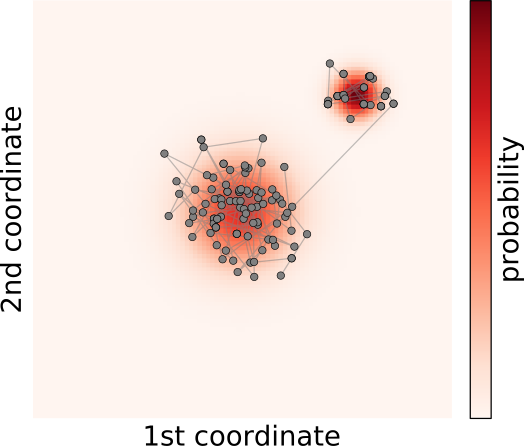
\includegraphics[width=0.8\textwidth]{images/dist_2d_chain}
    \end{column}
    \begin{column}{0.4\textwidth}
      Unlucky us:\\
      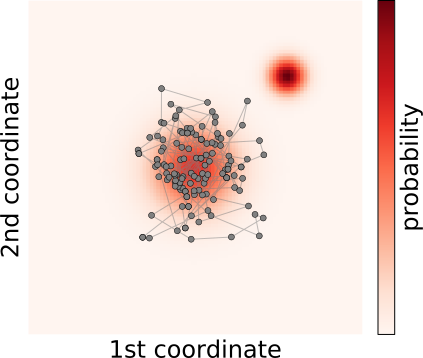
\includegraphics[width=0.8\textwidth]{images/dists_2d_chain_stuck}
    \end{column}
  \end{columns}
  \bigskip
  In higher dimensions: long time until all modes are discovered, if ever
\end{frame}

\begin{frame}
  \frametitle{Replica Exchange}
  Simulate ``flatter'' versions of probability distribution\only<1>{...}\only<2-3>{ and exchange states between Markov chains}\\
  \begin{center}
    \includegraphics<1>[width=0.5\textwidth]{movies_lowq/re/tmp00003}
    \includegraphics<2>[width=0.5\textwidth]{movies_lowq/re/tmp00004}
    \includegraphics<3>[width=0.5\textwidth]{movies_lowq/re/tmp00005}
  \end{center}
\end{frame}

\begin{frame}
  \frametitle{Replica Exchange: choosing swap partners}
  Choose swap partners such that all replicas are connected, for example:
  \begin{center}
    \includegraphics[width=0.6\textwidth]{images/good_swap_strategy}
  \end{center}
\end{frame}

\begin{frame}[fragile]
  \frametitle{Replica Exchange: acceptance criterion (informal motivation)}
  Plain exchanges disturb equilibrium distributions\\
  $\rightarrow$ correct with acceptance criterion\\
  \begin{center}
  \begin{tikzcd}[column sep=2cm, row sep=normal]
    {p_i(x)\mathrm{:} \ \ \ } x_{k-1}^i \arrow[r] & x_k^i \onslide*<1>{\arrow{dr}{p_{i\rightarrow j}}} & x_{k+1}^i \arrow[r]  & x_{k+2}^i\\
    {p_j(x)\mathrm{:} \ \ \ } x_{k-1}^j \arrow[r] & x_k^j \onslide*<2>{\arrow{ur}{p_{j\rightarrow i}}} & x_{k+1}^j \arrow[r,""]  & x_{k+2}^j
  \end{tikzcd}
  \end{center}
  \bigskip
  \begin{columns}
    \begin{column}{0.48\textwidth}
      Probability of accepting $x_k^i$ as ($k+1$)st state of $p_j(x)$ chain:
      \begin{equation*}
        p_{i\rightarrow j}=\frac{p_j(x_k^i)}{p_j(x_k^j)}
      \end{equation*}
    \end{column}
    \begin{column}{0.48\textwidth}
      \onslide<2>{Probability of accepting $x_k^j$ as ($k+1$)st state of $p_i(x)$ chain:
        \begin{equation*}
          p_{j\rightarrow i}=\frac{p_i(x_k^j)}{p_i(x_k^i)}
        \end{equation*}
      \end{column}
    \end{columns}
  }
\end{frame}

\begin{frame}[fragile]
  \frametitle{Replica Exchange: acceptance criterion (informal motivation)}
  Multiply $p_{i\rightarrow j}$ and $p_{j\rightarrow i}$:
  \begin{tcolorbox}[title=General acceptance criterion]
    \begin{equation*}
      p_{\mathrm{acc}}= \mathrm{min}\Bigg\{1, \frac{p_i(x^j)}{p_i(x^i)} \times \frac{p_j(x^i)}{p_j(x^j)}\Bigg\}
    \end{equation*}
  \end{tcolorbox}
  \begin{columns}
    \begin{column}[T]{0.5\textwidth}
      Common case with $p_i(x)\propto \mathrm{e}^{-\beta_i E(x)}$:
      \begin{equation*}
        p_{\mathrm{acc}} = \mathrm{min}\bigg\{1, \mathrm{e}^{(\beta_i-\beta_j)(E(x^i)-E(x^j))}\bigg\}
      \end{equation*}
    \end{column}
    \begin{column}[T]{0.43\textwidth}
      \begin{tcolorbox}[title=Physics terms]
        $\beta$: ``inverse temperature''\\
        $E(x)=-\log p(x)$: ``energy''
      \end{tcolorbox}
    \end{column}
  \end{columns}
  \bigskip
  \textcolor{red}{The more different $\beta_i$ and $\beta_j$, the lower $p_{\mathrm{acc}}$!}
\end{frame}

\begin{frame}
  \frametitle{Replica Exchange: life of a state}
  Single states perform a random walk on a temperature ladder:
  \begin{center}
    \includegraphics[width=0.5\textwidth]{images/state_trajectories}
  \end{center}
  Diffusion process: time to traverse ladder scales with $\sqrt{\#\mathrm{\ replicas}}$
\end{frame}

\begin{frame}
  \frametitle{Replica Exchange: TF Probability implementation}
\end{frame}

\begin{frame}
  \frametitle{Application: Bayesian determination of chromatin structures}
\end{frame}

\begin{frame}
  \frametitle{Application: Bayesian determination of chromatin structures}
\end{frame}

\begin{frame}
  \frametitle{Waste recycling: multiple histogram reweighting}
\end{frame}

\begin{frame}
  \frametitle{Model comparison}
\end{frame}


\begin{frame}[label=evidence_frame]
  \frametitle{Evidence}
  \onslide<1->
  \begin{description}
  \item[$p(D) = \int \d x\ p(D|x)p(x)$:]\hfill \\
    normalization constant (long story...)
  \end{description}
  In our case:
   \begin{tikzpicture}
     \node (content2) at (0,0) {\begin{minipage}{\paperwidth}
  \begin{align*}
    p(k=1) &= \int_0^1 \d b\ L(k=1|b) p(b) \\
           &= \int_0^1 \d b\ \left.\mathrm{Bernoulli}(k; b) \times \mathrm{Beta}(k;\alpha=2, \beta=2)\right\vert_{k=1} \\
           &= \int_0^1 \d b\ \left.b^{k}(1-b)^{k-1} \frac{b (1-b)}{\frac{\Gamma(2)\Gamma(2)}{\Gamma(4)}}\right\rvert_{k=1} \\
           &\;\;\vdots \\
           &=\frac{1}{2}
  \end{align*}\end{minipage}};
     \onslide<2->\node[align=center,red,font={\fontsize{50}{50}\bfseries}, rotate=45] at (content2.center) {YIKES};
   \end{tikzpicture}
\end{frame}

\begin{frame}
  \frametitle{Real-world Bayesian data analysis}
  \begin{columns}
    \begin{column}[T]{0.48\textwidth}
      In real problems: non-standard, difficult posterior distributions\\
    \end{column}
    \begin{column}[T]{0.48\textwidth}
      \includegraphics[width=0.5\textwidth]{images/2d_multimodal}
    \end{column}
  \end{columns}
  \begin{columns}
    \begin{column}{0.6\textwidth}
      \begin{tcolorbox}[title=Probabilistic programming libraries]
        Allow to
        \begin{itemize}
        \item programmatically define a statistical model
        \item sample from arbitrary posterior distributions
        \item run quality checks
        \end{itemize}
      \end{tcolorbox}
    \end{column}
    \begin{column}{0.38\textwidth}
      \vfill
      Examples:
      \begin{itemize}
      \item PyMC3
      \item Stan
      \item TensorFlow Probability
      \item ...
      \end{itemize}
      \vfill
    \end{column}
  \end{columns}
\end{frame}

\begin{frame}
  \frametitle{Interlude: real-world issues}
  In reality, probability distributions often
  \begin{itemize}
  \item of non-standard form
  \item are multidimensional
  \item have highly correlated random variables
  \item are known only up to a normalization constant
  \end{itemize}
  Consequences:
  \begin{itemize}
  \item analytical evaluation of expectation values is impossible
  \item naïve sampling approaches are inefficient (curse of dimensionality)
  \end{itemize}
  \begin{columns}
    \begin{column}[T]{0.33\textwidth}
      \adjustbox{width=.9\textwidth}{
        \includegraphics{images/normalized_unnormalized_normal}
      }
    \end{column}
    \begin{column}[T]{0.63\textwidth}
      \includegraphics[width=0.35\textwidth]{images/dists_multi_grid}
      \includegraphics[width=0.35\textwidth]{images/dists_2d}
    \end{column}
  \end{columns}
\end{frame}

\end{document}
